\documentclass[a4paper, openany, ragged2e]{book}
\usepackage{ucs}
\usepackage{ifluatex}
\ifluatex
\usepackage[utf8x]{luainputenc}
\else
\usepackage[utf8x]{inputenc}
\fi
\usepackage{enumerate}
\usepackage{a4wide}
\usepackage[automark]{scrpage2}
\pagestyle{scrheadings}
\usepackage{amssymb}
\usepackage{ulem}
\usepackage{graphicx}
\usepackage[ngerman]{babel}
\usepackage{amsmath, amssymb, amstext, amsfonts, mathrsfs}
\usepackage[procnames]{listings}
\usepackage{color}
\usepackage{titlesec}
\usepackage{multicol}
\usepackage{listings}
\usepackage{pdfpages}
\usepackage{qtree}
\usepackage{pgfplots}
\usepackage{polynom}
%Package für euro Zeichen
\usepackage{eurosym}
\titleformat*{\section}{\large\bfseries}
\clearscrheadfoot
\usepackage{wasysym} %Fuer den Blitz
\lstdefinestyle{javaStyle}{%
	basicstyle={\small},
	language=Java,
	numbers=left,
	showstringspaces=false,
	%keywordstyle={\color{kwcolor}\bfseries},
	%stringstyle={\color{stringcolor}},
	commentstyle={\color{commentcolor}},
	tabsize=4,
	breaklines=true,
	%cmathescape=true,
	escapeinside=||
}
\lstnewenvironment{code}
	{\lstset{style=javaStyle}}
	{}
\newcommand{\codeFile}[1]{\lstinputlisting[style=javaStyle]{#1}}

\usepackage{todonotes}
\usepackage{hyperref}
\hypersetup{%
  colorlinks=false,% hyperlinks will be black
  linkbordercolor=blue,% hyperlink borders will be red
  pdfborderstyle={/S/U/W 1}% border style will be underline of width 1pt
}
\usepackage{listings,xcolor}
\usepackage{inconsolata}

\usepackage{float}

\title{%
  Dokumentation Programmierprojekt SS 16 \\ 
  \large Arbeitsbereich: Kommunikationsnetze 
  }


\author{Finn Ickler, Steffen Lindner, Dominik Spoerle, Maximillian Pfister \\ Betreuer: Wolfgang Braun}

\def\F{$\mathcal{F}$}
\def\mF{\mathcal{F}}
\def\pm{\par \medskip}
\newcommand{\tb}[1]{\textbf{#1}}

% Numberroomes
\newcommand{\N}{\mathbb{N}}
\newcommand{\R}{\mathbb{R}}
\newcommand{\Z}{\mathbb{Z}}
\newcommand{\Q}{\mathbb{Q}}
\newcommand{\C}{\mathbb{C}}

\newcommand{\T}{\mathcal{T}}
\newcommand{\Lm}{\mathbb{L}}

% Arrows
\newcommand{\ra}{\rightarrow}
\newcommand{\Ra}{\Rightarrow}

% Symbols
\newcommand{\Lr}{\Leftrightarrow}
\newcommand{\Th}{\Theta}
\newcommand{\Om}{\Omega}
\newcommand{\Fa}{\mathcal{F}}
\newcommand{\Po}{\mathcal{P}}
\newcommand{\oo}{\mathcal{O}}

% Listings
\newcommand{\ba}{\begin{enumerate}[label=(\alph*)]}
\newcommand{\ea}{\end{enumerate}}
\newcommand{\bi}{\begin{itemize}}
\newcommand{\ei}{\end{itemize}}

% Sectioning
\newcommand{\subs}[1]{\subsection*{#1}}
\newcommand{\sss}[1]{\subsubsection*{#1}}

% Code style
\lstdefinelanguage{Scheme}{
  morekeywords=[1]{define, define-syntax, define-macro, lambda, define-stream, stream-lambda},
  morekeywords=[2]{begin, call-with-current-continuation, call/cc,
    call-with-input-file, call-with-output-file, case, cond,
    do, else, for-each, if,
    let*, let, let-syntax, letrec, letrec-syntax,
    let-values, let*-values,
    and, or, not, delay, force,
    quasiquote, quote, unquote, unquote-splicing,
    map, fold, syntax, syntax-rules, eval, environment, query },
  morekeywords=[3]{import, export},
  alsodigit=!\$\%&*+-./:<=>?@^_~,
  sensitive=true,
  morecomment=[l]{;},
  morecomment=[s]{\#|}{|\#},
  morestring=[b]",
  basicstyle=\small\ttfamily,
  keywordstyle=\bf\ttfamily\color[rgb]{0,.3,.7},
  commentstyle=\color[rgb]{0.133,0.545,0.133},
  stringstyle={\color[rgb]{0.75,0.49,0.07}},
  upquote=true,
  breaklines=true,
  breakatwhitespace=true,
  literate=*{`}{{`}}{1}
}

\lstset{
  language        = php,
  basicstyle      = \small\ttfamily,
  keywordstyle    = \color{dkblue},
  stringstyle     = \color{red},
  identifierstyle = \color{dkgreen},
  commentstyle    = \color{gray},
  emph            =[1]{php},
  emphstyle       =[1]\color{black},
  emph            =[2]{if,and,or,else},
  emphstyle       =[2]\color{dkyellow}
  }



\definecolor{dkgreen}{rgb}{0,.6,0}
\definecolor{dkblue}{rgb}{0,0,.6}
\definecolor{dkyellow}{cmyk}{0,0,.8,.3}

\setcounter{secnumdepth}{2}
\setcounter{tocdepth}{4}

\renewcommand{\chaptername}{}
\renewcommand{\contentsname}{Inhaltsverzeichnis}
\titleformat{\chapter}
  {\Large\bfseries} % format
  {}                % label
  {0pt}             % sep
  {\huge}           % before-code


\setlength{\parskip}{0pt}
\setlength{\parindent}{0pt}
\setlength{\skip\footins}{0.5cm}

\usepackage[left=26mm,top=15mm,right=26mm,bottom=15mm]{geometry}

\ofoot{\pagemark}

\begin{document}
\maketitle

\tableofcontents

\chapter{Beschreibung der Software}

\section{Grundsturktur}

\chapter{Installationsanleitung}

\subsection{Systemanforderungen}


Unsere Software benötigt folgende Komponenten:

\begin{itemize}
	\item Apache Version 2.0 (mit aktiviertem mod\_rewrite) oder höher bzw. nginx 0.8.42 oder höher oder einen anderen Webserver der Url rewriting unterstützt
	\item PHP 5.2 oder höher (für Smarty)
	\item PHP-Erweiterung cURL	
\end{itemize}

\subsection{Konfiguration}

Jegliche (vom Nutzer vornehmbare) Konfiguration wird in der \textit{mainConfig.php} innerhalb des \textit{config} Verzeichnisses vorgenommen.

\pm

Dabei ist besonders der bereits angesprochende \textit{basepath} für den Nutzer interessant. Jenachdem, ob unsere Software in einem Unterverzeichnis aufgerufen wird (beispielsweise www.meineDomain.de/unterverzeichnis/) oder nicht, muss der \textit{basepath} entsprechend angepasst werden.

\begin{figure}[h!]
	\begin{lstlisting}[language=R]
	Config::set('basepath','unterverzeichnis');
	\end{lstlisting}
	\caption{Beispiel Basepath zur Konfiguration unserer Software}
\end{figure}

Innerhalb der \textit{mainConfig.php} lassen sich noch weitere Parameter einstellen, wie beispielsweise das Verzeichnis, in dem die Routen liegen (für das URL - Template-Matching), oder auch wie viele Kategorien / User pro Seite angezeigt werden sollen.

\subsection{Installation}

Die Installation gestaltet sich sehr einfach. Nachdem die Dateien in das gewünschte Verzeichnis kopiert wurden muss lediglich noch die Konfiguration des \textit{basepaths} durchgeführt werden (siehe Abschnitt Konfiguration).

\pm

Damit alle Anfragen auch an die \textit{index.php} weitergeleitet werden bedarf es allerdings noch einer Anpassung, die nun exemplarisch für Apache und nginx (unter unixoiden Systemen) beschrieben werden soll.

\subsubsection{Apache}

Zunächst muss geprüft werden, ob \textit{mod\_rewrite} geladen wurde. Dazu kann das folgende bash Kommando genutzt werden: 

\begin{figure}[H]
	\begin{lstlisting}
		apachectl -M | grep 'rewrite_module'
	\end{lstlisting}
	\caption{Überprüfung ob \textit{mod\_rewrite} geladen wurde}
\end{figure}

Da es sich bei \textit{mod\_rewrite} um ein ASF\footnote{ASF: Apache software foundation: Standardmodul} Modul handelt, ist es in der Regel automatisch installiert. Wird es nicht gefunden, so muss es für gewöhnlich lediglich aktiviert werden:

\begin{figure}[H]
	\begin{lstlisting}
		a2enmod rewrite
	\end{lstlisting}
	\caption{Aktivierung von \textit{mod\_rewrite}}
\end{figure}

Nun muss in der httpd.conf (bzw. einer geladenen Konfiguration von Apache) für das Verzeichnis, in dem unsere Software liegt, das Umschreiben der URL erlaubt werden. Dazu genügt ein Eintrag wie folgt:

\begin{figure}[H]
	\begin{lstlisting}
<Directory "/var/www/unterverzeichnis/">
	AllowOverride All
</Directory>	
	\end{lstlisting}
	\caption{Erlaube das Umschreiben der URL für ein gewünschtes Verzeichnis}
\end{figure}

Anschließend muss in der \textit{.htaccess}-Datei im Wunschverzeichnis die \textit{RewriteBase} angepasst werden. Für das gegebene Beispiel würde folgen:

\begin{figure}[H]
	\begin{lstlisting}
	RewriteBase /unververzeichnis	
	\end{lstlisting}
	\caption{Anpassung der RewriteBase in der \textit{.htaccess}}
\end{figure}

\subsubsection{Nginx}

Wird nginx verwendet, so muss das '\textit{ngx\_http\_rewrite\_module}\footnote{NGINX Rewrite: http://nginx.org/en/docs/http/ngx\_http\_rewrite\_module.html}' installiert sein. Anschließend muss in der nginx.conf folgender Eintrag ergänzt werden:

\begin{figure}[H]
	\begin{lstlisting}
location /unterverzeichnis {
  alias /srv/ss16-web/htdocs;
  index index.php;
  try_files $uri $uri/ /ss16-web/trunk/index.php?$query_string;
}	
	\end{lstlisting}
	\caption{Beispielhafte nginx.conf zur URL Umleitung}
\end{figure}

wobei die Pfade nach der tatsächlichen Struktur anzupassen sind.

\subsection{Inbetriebnahme}

Ab diesem Moment ist unsere Software einsatzbereit.



























\chapter{Bedienungsanleitung}

\section{Kurzbeschreibung der Software}

\textbf{WolfGang} ist eine Video-Streaming-Dienst, der im Rahmen des Software-Projekts 2016 an der Universität Tübingen entwickelt wurde. Das Videoportal soll den Benutzern das kostenloses Anschauen, Verwalten und Hochladen von Videos ermöglichen.


\section{Hinweise zum ersten Start}
Um alle Funktionen der Website nutzen zu können (Drop-Down-Menü für die Navigation bzw. für den Login), muss \textbf{Javascript} aktiviert sein. \\
Um alle Features unserer Seite zu erhalten, sollten sie sich bei ihrem ersten Besuch einen Account anlegen und sich mit diesem Anmelden. Dann können sie eigene Playlisten erstellen und Videos bewerten und kommentieren. \\
Falls sie sich gut verhalten, werden sie womöglich zu einem priviligierten Benutzer befördert und sie können Videos auf die Seite hochladen und dieses verwalten. \\


\section{Verfügbare Funktionen in Abhängigkeit der Benutzerrechte}
Die Benutzer der Website werden in Gruppen in Abhängigkeit ihrere Rechte eingeteilt. \\ Gäste, die keinen Account besitzen, sind User der Gruppe 1. \\
Ein eingeloggter Benutzer gehört zur  Gruppe 2. \\
Von einem Admin priviligierte Benutzer gehören zur Gruppe 3, \\
die Admins bilden die Gruppe 4. \\
Daraus ergeben sich für die verschiedenen Funktionen der Website folgende Berechtigungen: \\
\par \medskip
\label{Rechte}
\begin{table}[h]
	\centering
	\begin{tabular}{l|c|c|c|c}
		Usergruppe & 1 & 2 & 3 & 4 \\
		\hline
		Account erstellen & $\checkmark$ & & &  \\
		Video,Playlist abspielen & $\checkmark$ & $\checkmark$ & $\checkmark$ & $\checkmark$  \\
		Playlist erstellen & & $\checkmark$ & $\checkmark$ &$\checkmark$  \\
		Playlist bearbeiten & & ($\checkmark$) & ($\checkmark$) & $\checkmark$ \\
		Playlist löschen & & ($\checkmark$) & ($\checkmark$) & $\checkmark$ \\
		Video bewerten und kommentieren & & $\checkmark$ & $\checkmark$ &$\checkmark$  \\
		Profil bearbeiten & & ($\checkmark$) & ($\checkmark$ ) & ($\checkmark$) \\
		Video hochladen & & & $\checkmark$ & $\checkmark$  \\
		Video zu Kategorie hinzufügen & & & ($\checkmark$) & $\checkmark$  \\
		Video von Kategorie löschen & & & ($\checkmark$) & ($\checkmark$)  \\
		Benutzer löschen & & & & $\checkmark$  \\
		Benuter-Rechte verwalten & & & & $\checkmark$  \\
		Kategorie erstellen,bearbeiten,löschen & & & & $\checkmark$ \\
		
	\end{tabular}\\
	\caption{Verfügbare Funktionen in Abhängigkeit von den Benutzerrechten}
\end{table}
\medskip

Eine eingeschränkte Berechtigung ($\checkmark$) bedeutet,dass die Aktion nur für eigene "Objekte" verfügbar ist. \\
Dies sind das eigene Profil, eigene Playlists oder eigene Videos.


\subsection{Grundstruktur}
Die Website ist in 3 Bereiche unterteilt: \\

\begin{figure}[ht]
\centering
  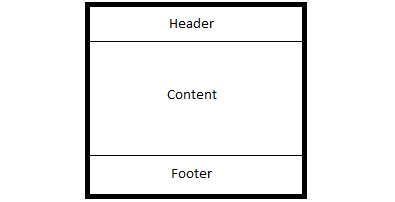
\includegraphics[width=0.33\textwidth]{./Includes/Bedienungsanleitung/Struktur.png}
	\caption{Grundstruktur}
\end{figure}
Der Header und der Footer sind dabei fest, der Content unterscheidet sich in Abhängigkeit der besuchten Unterseite. \\
Im weiteren werden die einzelnen Bereiche erklärt - möchten sie etwas genaueres über eine gewisse Funktion wissen, drücken sie \hyperref[Functions]{hier}
\subsubsection{Header}
\begin{figure}[ht]
\centering
  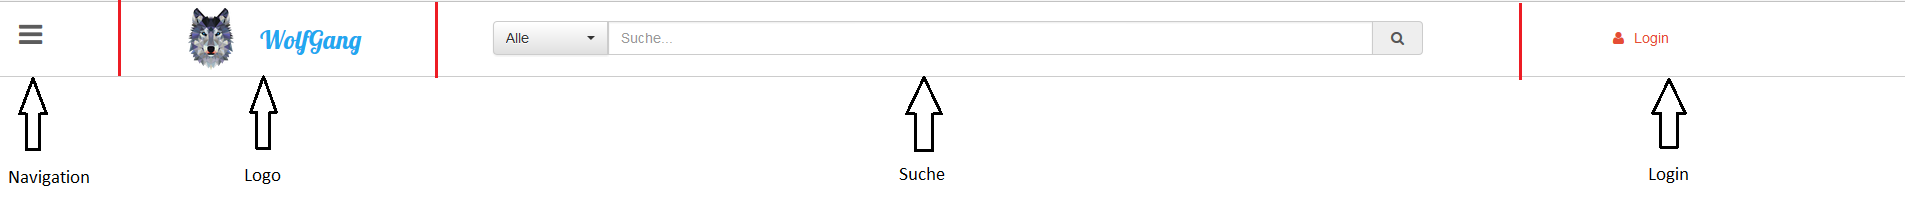
\includegraphics[width=1\textwidth]{./Includes/Bedienungsanleitung/header.png}
	\caption{Header-Unterteilung}
\end{figure}


\begin{enumerate}
\item \textbf{Navigation} \\
Die Navigation ist ein Drop-Down-Menü und enthält eine Verlinkung auf alle wichtigen Seiten\\
(Dabei werden nur die Seiten angezeigt, die der Benutzer auch besuchen kann). \\
\begin{figure}[ht]
\centering
  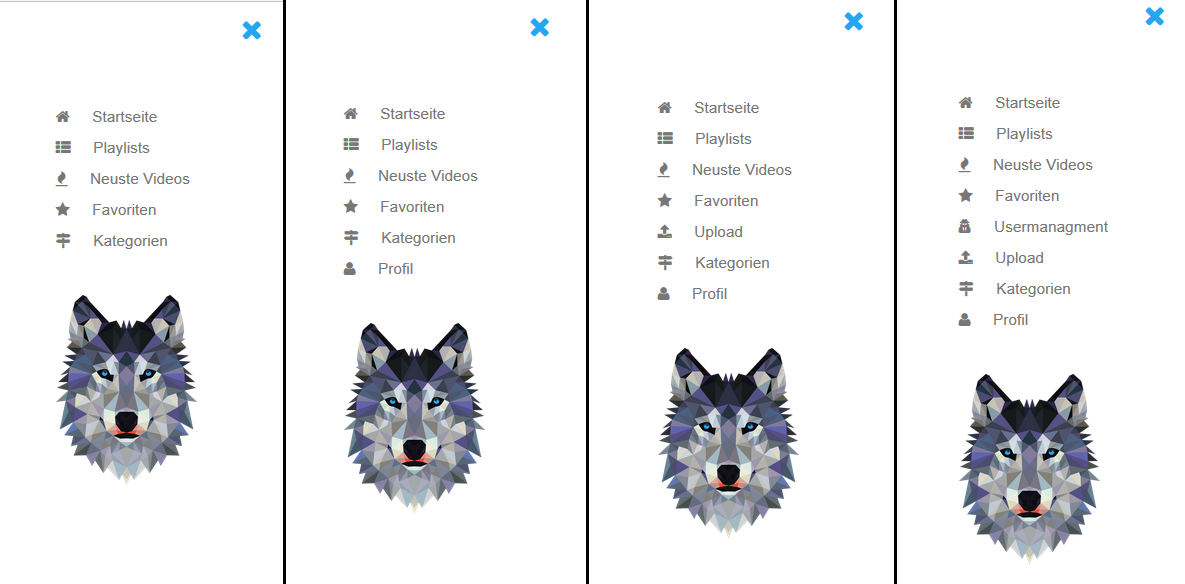
\includegraphics[width=1\textwidth]{./Includes/Bedienungsanleitung/navigationen.png}
	\caption{Ansicht der Navigationen mit verschiedenen Rechten (v.l. 1,2,3,4)}
\end{figure}


Versucht man, eine Seite über eine Manipulation der URL zu besuchen, für die man keine Berechtigung besitzt, so findet eine Weiterleitung zur Fehlerseite statt.
\item \textbf{Schriftzug und Logo} \\
Das Logo, dass natürlich auf keiner Website fehlen darf, ist gleichzeitig noch ein Link zur Startseite.
\item \textbf{Suche} \\
Im Suchfeld kann nach einem Video, einer Playlist oder einer Kategorie gesucht werden. Näheres wird im Unterpunkt \hyperref[video:suchen]{Video suchen} erläutert.
\item \textbf{Login}
Der Log-In Bereich enthält Informationen darüber, ob mal angemeldet ist und einen Button, mit dem man sich ggf. anmelden kann. Näheres zur Log-In Funktion finden sie unter \hyperref[login]{Wie melde ich mich an?}
\end{enumerate}
\medskip

\subsubsection{Content}
Der Content ist abhängig von der besuchten Unterseite und stellt zum Beispiel die Videoansicht, die Profilverwaltung oder die Playlistverwaltung dar.

\subsubsection{Footer}
%\begin{figure}[ht]
%\centering
% 
\includegraphics[width=1\textwidth]{./Includes/Bedienungsanleitung/footer.png}
%	\caption{Fußzeile}
%\end{figure}


Der Footer bietet neben dem farblichen Kontrast zur Seite einen Link zum Impressum (hierfür wurde das offizielle Impressum der Uni-Tübingen verwendet), einen Link zur Dokumentation der Software sowie einen Link zu den Social-Medias von \textbf{Wolfgang}.
\par \medskip
Desweiteren gibt es auf Unterseiten, welche durch die Darstellung vieler Videos eine große Höhe besitzen, einen Top-Button, der zum Anfang(nach oben) ''zurückspringt''. \\
Statusinformationen (wie Fehlermeldungen oder ähnlichem) des Servers werden rechts unten als Inhalt einer Notify-Box angezeigt, die nach einigen Sekunden wieder verschwindet.
\begin{figure}[ht]
\centering
  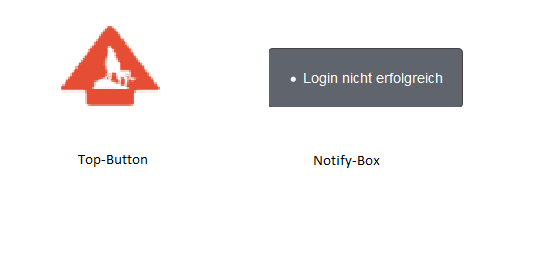
\includegraphics[width=0.5\textwidth]{./Includes/Bedienungsanleitung/topnotify.png}
	\caption{Top-Button und Notify-Box am Beispiel des fehlgeschalagenen Log-Ins}
\end{figure}

\subsubsection{Navigation auf der Seite}
Verfügbare Seiten und deren Inhalte:
\begin{enumerate}[a)]
	\item Startseite: Meist gesehene Videos (im Headerbereich), Zufälliges Video, Video of the Week, Kategorien Tag Cloud
	\item Playlists: Neuste Playlist, Top Rated Playlist, eigene Playlisten, abonnierte Playlisten, alle Playlisten
	\item Neuste Videos: neuste Videos, meist gesehenes Video, alle Videos
	\item Favoriten: Populäre Videos, meist gesehenes Video, Videos mit bestem Rating, alle Videos
	\item Usermanagement: Übersicht aller User, Rechteänderungen von Usern, Löschen von Usern
	\item Upload: Video Upload
	\item Kategorien: Übersicht Kategorien, Kategorie und enthaltene Videos
	\item Profil: Nutzerprofil - Änderungen von Nutzerdaten, Übersicht eigene Videos, eigene Playlists
\end{enumerate}

\paragraph{Navigationsmittel}
\begin{enumerate}[a)]
	\item Hauptmenü links: kann per Klick auf das Menü-Icon links oben geöffnet werden
	\item Suchfunktion (suchen nach Videos, Playlisten, Kategorien)
	\item Logo: Link zur Startseite
	\item Video- und Playlisten-Play-Buttons: führen zu entsprechenden Detailseite
	\item auf einer Seite: Top-Button/ Pfeil rechts unten, scrollt zum Seitenanfang
\end{enumerate}
 

\subsection{Funktionen}
\label{Functions}
\subsubsection{Header Funktionen}

\paragraph{Profil erstellen}
~ \\
\begin{figure}[ht]
\centering
  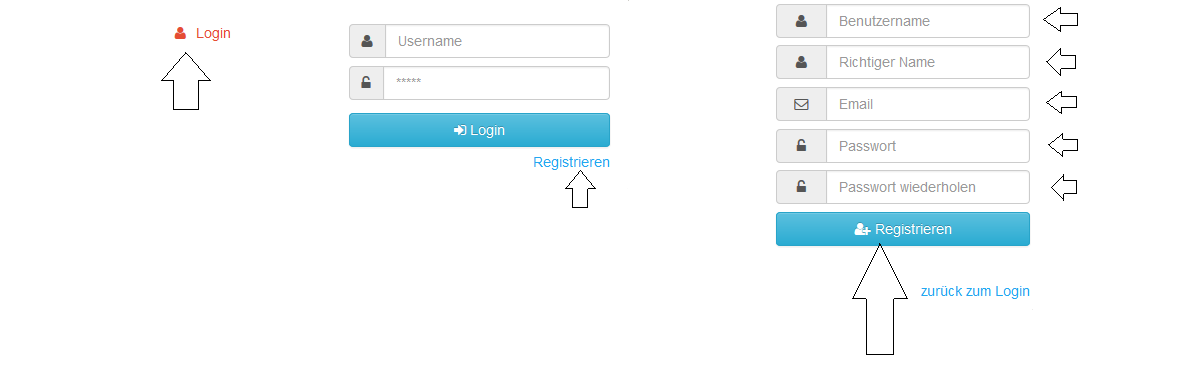
\includegraphics[width=1\textwidth]{./Includes/Bedienungsanleitung/registrierung.png}
	\caption{LogIn-Button \quad LogIn-Form mit Link zur Registrierung \quad Registrierung-Form}
\end{figure}

1. Drücken sie rechts im Header auf den \textit{Log-In Button}. Es öffnet sich das Log-In-Menü. \\
2. Drücken sie den Link  \textit{Registierung}, der sich am unteren rechten Rand des Log-In-Menüs befindet. Es öffnet sich ein weiteres Fenster. \\
3. Tragen sie in die einzelnen Felder die geforderten Daten ein und klicken sie den Bestätigungsbutton. Bekommen sie als Antwort des Servers "Ihre Registierung war erfolgreich" so wurde ihr Account erfolgreich registriert. Falls es eine andere bzw. keine Benachrichtigung gibt, versuchen sie die Lösungen \hyperref[probleme]{hier}

\paragraph{Anmeldung}
\label{login}
\begin{figure}[ht]
\centering
  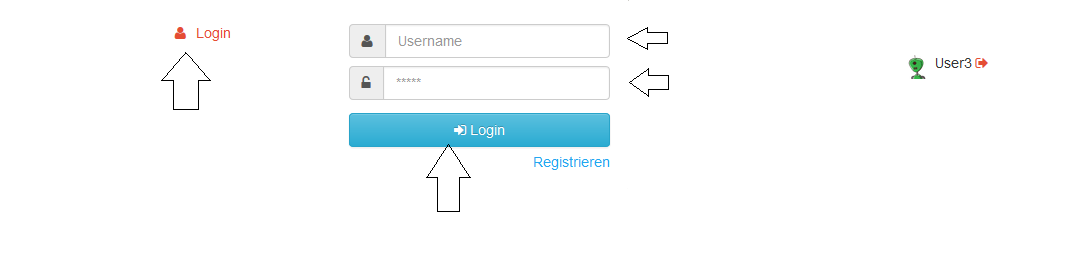
\includegraphics[width=1\textwidth]{./Includes/Bedienungsanleitung/login.png}
	\caption{ Login-Button \quad  Login-Felder \quad  Angemeldeter Benutzer mit Logout-Button}
\end{figure}
Besitzen sie einen Account, so können sie sich wie folgt anmelden: \\
(Wie sie einen neuen Account erstellen finden sie unter: \hyperref[Functions]{Wie erstelle ich einen Account})  \\
1. Drücken sie rechts im Header auf den \textit{Log-In Button}. Es öffnet sich das Log-In-Menü. \\
2. Zum Einloggen geben sie bitte ihren Benutzernamen und das zugehörige Passwort ein. \\
3.War die Aktion erfolgreich, so wird die Seite neu geladen und sie werden im Header mit ihrem Namen begrüßt. Bekommen sie als Rückmeldung "Login nicht erfolgreich" so war entweder das Passwort falsch oder es existiert der Benuter nicht.

\paragraph{Suchfunktion}
\label{video:suchen}
Die Suche eines Videos ist von überall über die Suchfunktion im Header möglich. \\ 1. Klicken sie dazu auf das Eingabefeld.\\
2. Geben sie ihre Suche ein\\
3. Bestätigen sie per Mouseclick auf den Suche-Button (oder per Enter). \\
Auf der Ergebnisseite können sie oben zwischen den gefundenen Videos,Kategorien und Playlists wechseln: \\
\begin{figure}[ht]
\centering
  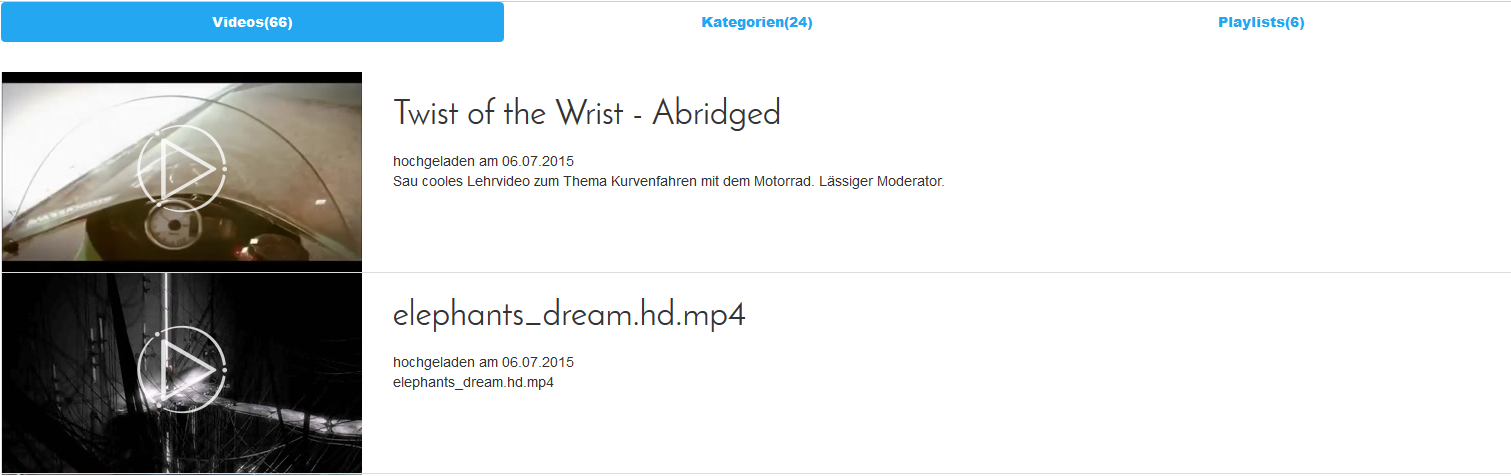
\includegraphics[width=1\textwidth]{./Includes/Bedienungsanleitung/suchergebniss.png}
	\caption{Suchergebnisse für den String ''A''}
\end{figure}

Während dem Eingeben werden ihnen bereits zutreffende Resultate mit dem zugehörigen Bereich(also ob es sich bei den Ergebnissen um Videos, Kategorien oder Playlisten handelt) angezeigt - diese können sie per Mouseclick auswählen. \\
\begin{figure}[ht]
\centering
  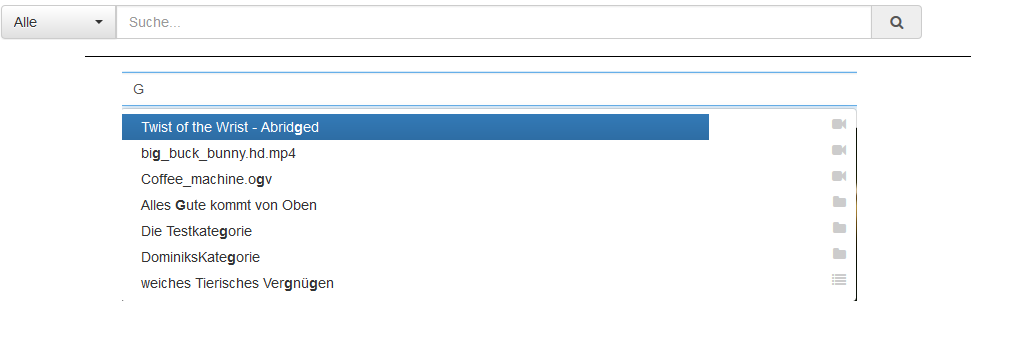
\includegraphics[width=1\textwidth]{./Includes/Bedienungsanleitung/ajaxsuche.png}
	\caption{Suchergebnisse des Suchstrings ''G''}
\end{figure}

\medskip
Rechts von dem Suchfeld könne sie vorab bereits ihre suche spezifizieren, wenn sie nach etwas Bestimmten suchen wollen.
\begin{figure}[ht]
\centering
  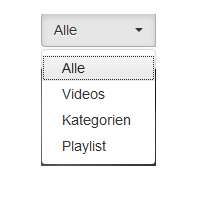
\includegraphics[width=0.2\textwidth]{./Includes/Bedienungsanleitung/searchreiter.png}
	\caption{Eingrenzung der Suche }
\end{figure}

\textit{Tipp}: Beginnt ihr Suchstring mit v: (bzw. c: oder p:), so wird automatisch nach dem zugehörigen Bereich (v - Video, c - Category, p - Playlist) gesucht, ohne dass sie dies im Reiter explizit auswählen müssen. \\

\subsubsection{Profil}

Das Profil bietet die Möglichkeit das Passwort und die persönlichen Daten (Email, Username, etc) zu ändern. Außerdem zeigt das Profil die von einem User hochgeladenen Videos und erstellten Playlisten an.

\begin{figure}[H]
	\centering
	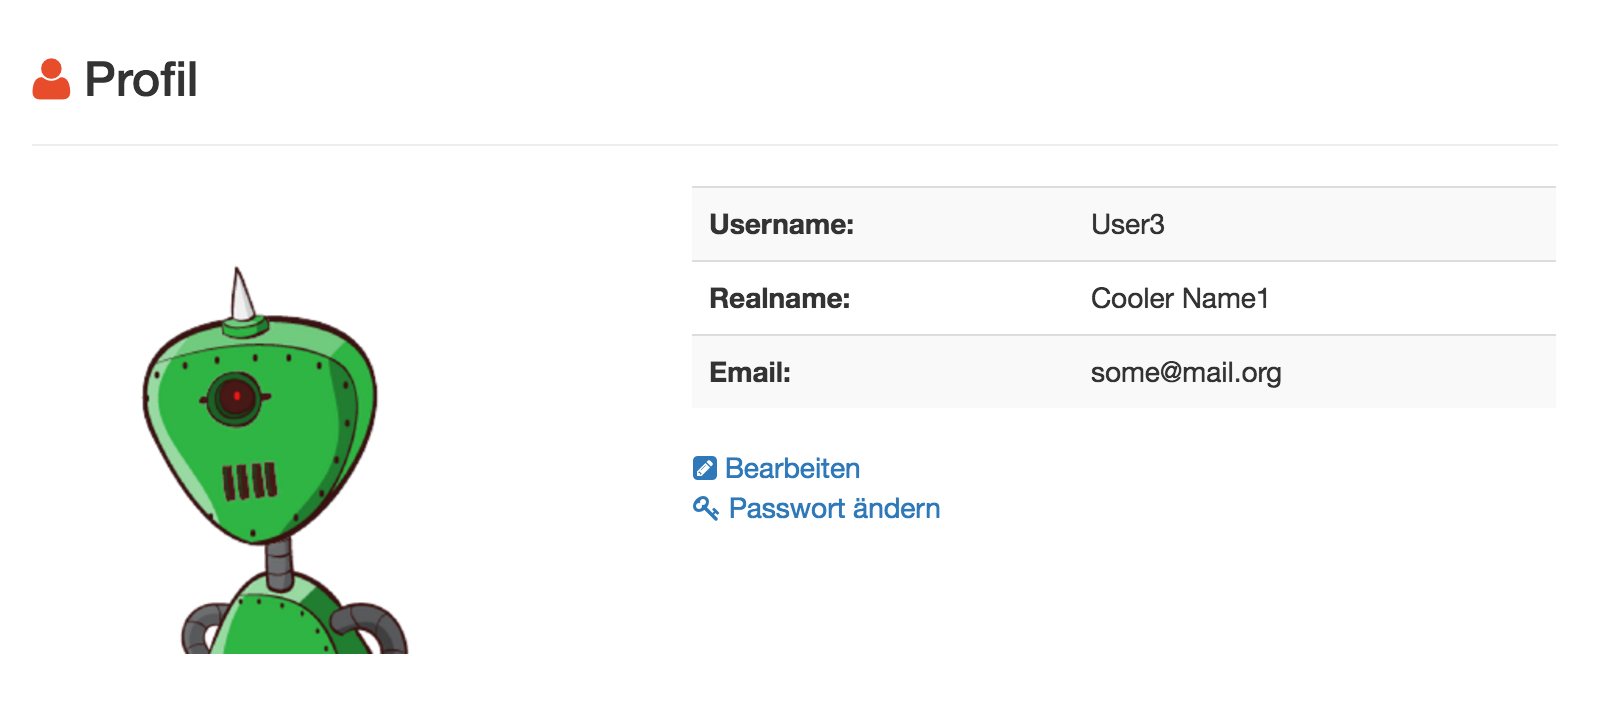
\includegraphics[width=0.9\textwidth]{Includes/Bedienungsanleitung/profil.png}
	\caption{Ansicht Profilseite}
\end{figure}

Über die Buttons Bearbeiten bzw. Passwort ändern können die Nutzerdaten geändert werden.

\begin{figure}[H]
	\centering
	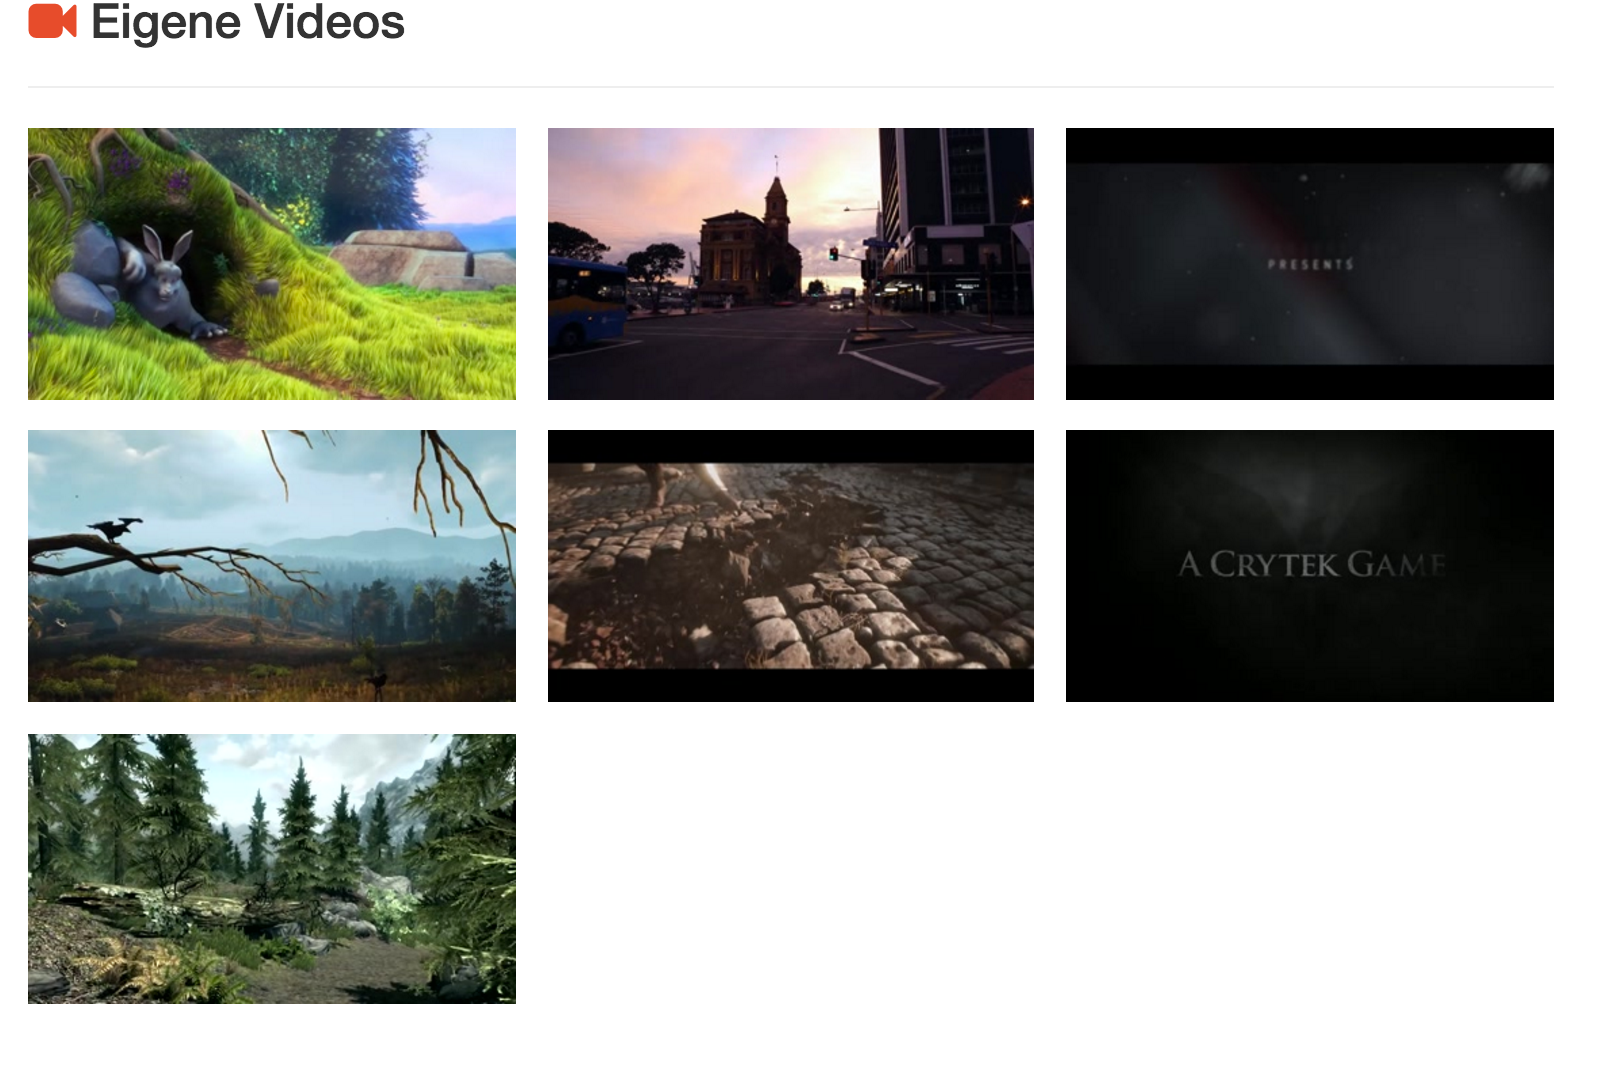
\includegraphics[width=0.9\textwidth]{Includes/Bedienungsanleitung/profil_own_video.png}
	\caption{Ansicht Profilseite eigene Videos}
\end{figure}

Fährt man über eines seiner eigenen Videos auf dem Profil, so kann man diese löschen (der Admin kann auch auf fremden Profilen Videos löschen).



\subsubsection{Videos verwalten}
Die Verwaltung von Videos ist registrierten Benutzern vorenthalten. Als Besucher ohne Login Zugang kann man alle existierenden Videos ansehen, dabei hat man mehrere Möglichkeiten Videos zu finden oder auf der Seite zu stöbern. 

\paragraph{Videos ansehen} 
~ \\ \\
Wenn Sie ein Video anschauen möchten, klicken Sie auf das Vorschaubild und sie werden zur Video-Detailansicht des Videos weitergeleitet. Dort stehen die normalen Funktionen eines Videoplayers, analog zum gängigen HTML5-Player, zur Verfügung:
\begin{itemize}
	\item Der Play/Pause-Button spielt das Video ab oder hält es an.
	\item Mithilfe der Lautstärkeregelung können sie die Lautstärke einstellen.
	\item Daneben befindet sich ein Button, um das Video zu maximieren (Full Screen Modus).
	\item Unter dem Video befinden sich verschieden Qualitätsstufen, in der sie das Video anschauen können (diese sind abhängig von der Qualität des Videos).
\end{itemize}

\begin{figure}[ht]
	\centering
	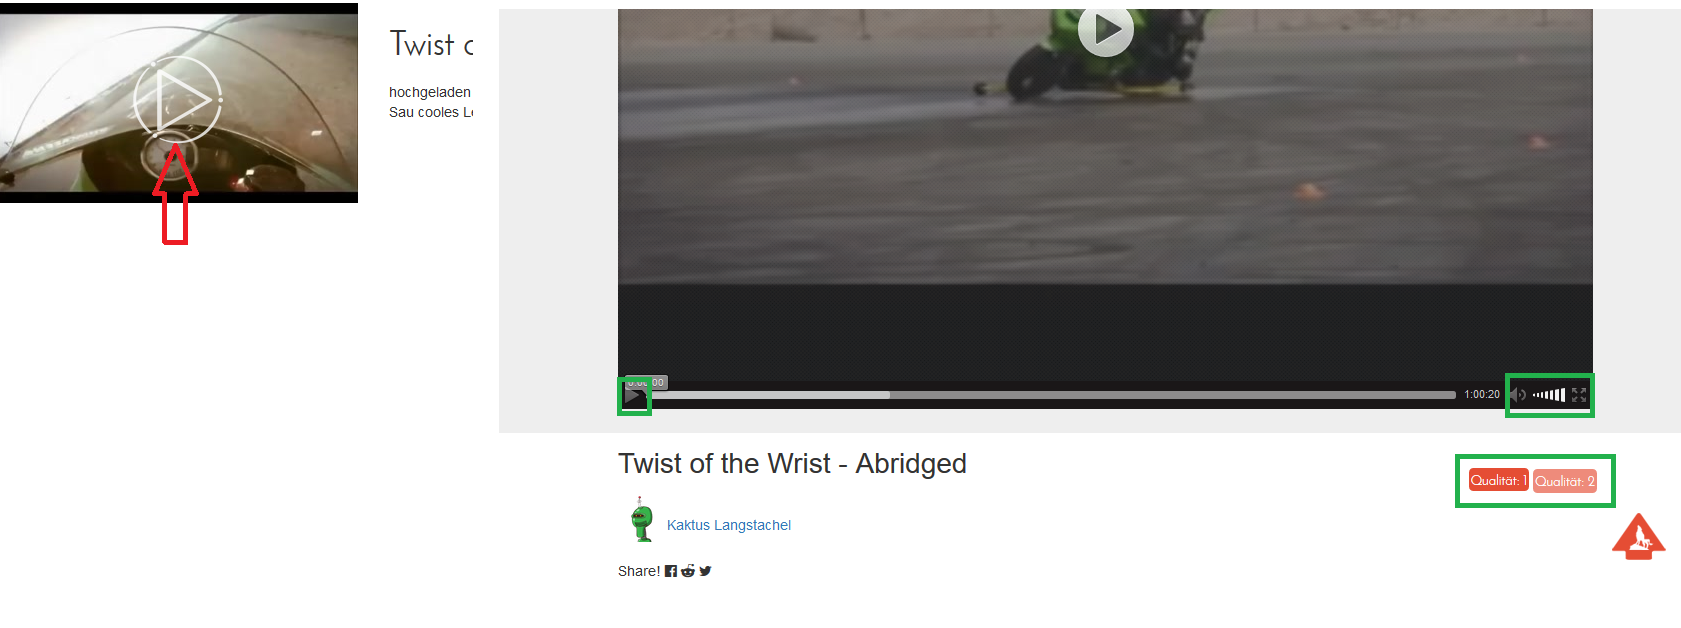
\includegraphics[width=1\textwidth]{./Includes/Bedienungsanleitung/videoansicht.png}
	\caption{Videoansicht des Videos ''Twist of the Wrist''}
\end{figure}

\paragraph{Video hochladen}
~ \\
Unter ''Upload'' können von einem eingeloggten Benutzern (ab Usergruppe 4) Videos hochgeladen werden. \\


\begin{figure}[h!]
	\centering
	
\includegraphics[width=1\textwidth]{./Includes/Bedienungsanleitung/upload.png}
	\caption{Ansicht Upload}
	\label{fig:somthing}
\end{figure}

\pm

{\bf Übersicht zu Abbildung 3.11}
\begin{enumerate}
	\item Feld für Drag'n Drop Eingabe von Video-Dateien, dabei kann immer nur 1 Datei hochgeladen werden. Zulässig sind dabei die Dateitypen: {\it mp4, mov, mpeg, wmv, avi, swf, flv, mpg}
	\item ''Browse-Button'' zum suchen von Video Dateien auf dem Computer.
	\item Name und Beschreibung des neuen Videos. Geben WolfGang-Besuchern nähere Infos zum Video. \\
	{\it keine Pflichtfelder}
\end{enumerate}

\begin{figure}[h!]
	\centering
	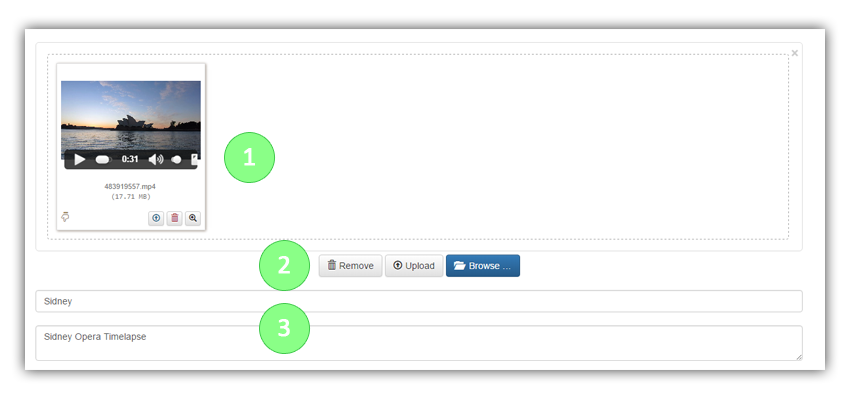
\includegraphics[width=1\textwidth]{./Includes/Bedienungsanleitung/upload_data.png}
	\caption{Ansicht Upload: nach dem Hinzufügen einer Videodatei}
	\label{fig:somthing}
\end{figure}

\pm

{\bf Übersicht zu Abbildung 3.12}
\begin{enumerate}
	\item Datei-Vorschau: hier ist das Abspielen des eingefügten Videos möglich, außerdem wird die Dateigröße angezeigt und das Element kann wieder aus dem Upload-Bereich gelöscht werden.
	\item Mit dem ''Remove''-Button kann die Datei aus dem Upload-Bereich gelöscht werden. \\
	Mit ''Upload'' wird das Video hochgeladen.\\
	Mit ''Browse'' wird erneut nach einer Datei auf dem Computer gesucht. Das ist nur dann möglich, falls die aktuelle Datei wieder aus dem Upload-Bereich gelöscht wurde.
	\item Name und Beschreibung können auch in diesem Zustand noch ergänzt werden.
\end{enumerate}

\pm

Wurde das Video hochgeladen, wird auf die Profilseite des Nutzers geführt. Hier können alle bereits hochgeladenen Videos eingesehen und auch wieder gelöscht werden. Mit einem Klick auf das entsprechende Video, kann es in der \hyperref[fig:video-detail]{Video-Detailansicht} angesehen werden.

\begin{figure}[h!]
	\centering
	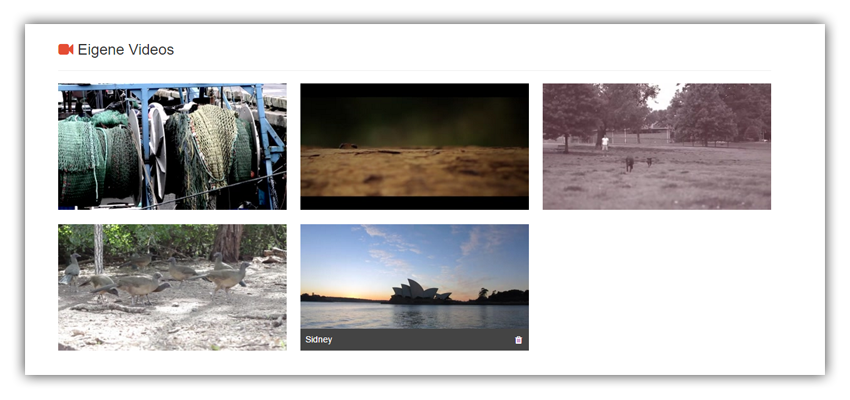
\includegraphics[width=1\textwidth]{./Includes/Bedienungsanleitung/profil_new-video.png}
	\caption{Ansicht Profil: nach dem Upload wird das neue Video hier mit allen bereits hochgeladenen Videos gelistet.}
	\label{fig:somthing}
\end{figure}

\clearpage

\paragraph{Video bearbeiten}
$\;$ \\ \\
Nur als eingeloggter Nutzer (ab Usergruppe 2) möglich. Ohne Login kann das Video lediglich abgespielt werden. Dabei sind Rating und Views des Videos sichtbar. \\

\begin{figure}[h!]
	\centering
	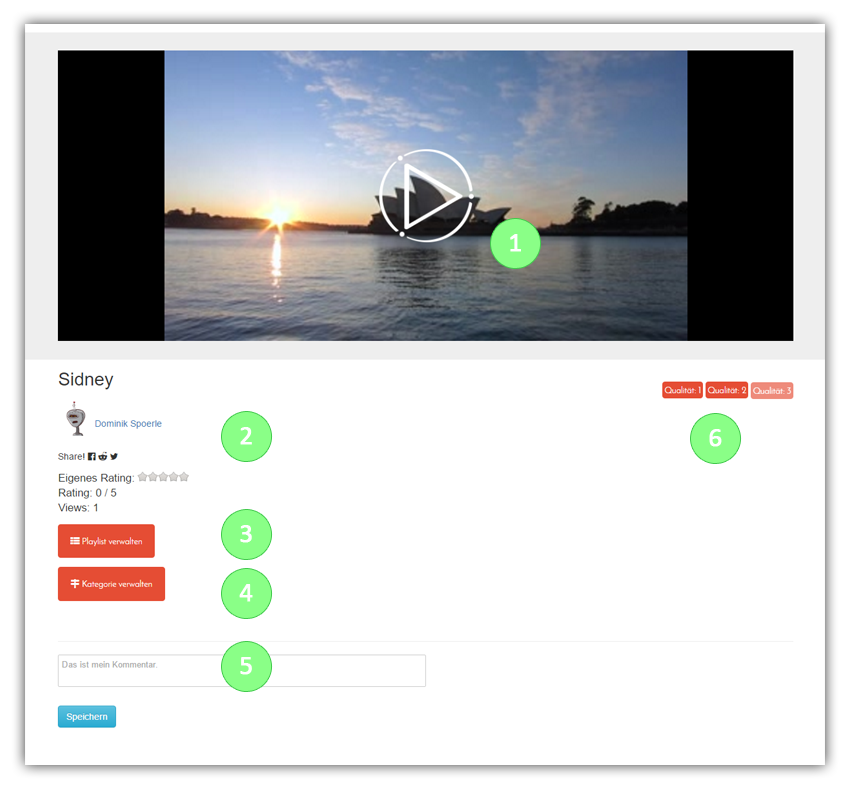
\includegraphics[width=1\textwidth]{./Includes/Bedienungsanleitung/video_overview.png}
	\caption{Ansicht Video: Video-Detailansicht}
	\label{fig:video-detail}
\end{figure}

{\bf Übersicht zu Abbildung 3.14}
\begin{enumerate}
	\item Video abspielen
	\item Video Informationen: Uploader-Name, Rating des eingeloggten Nutzers, Gesamtrating, Views
	\item Playlist verwalten: das Video kann zu einer Playlist hinzugefügt oder von einer Playlist entfernt werden.
	{\bf Hinweis:} das ist nur für Playlists des eingeloggten Nutzers möglich.
	\item Kategorie verwalten: das Video kann zu einer Kategorie hinzugefügt oder von einer Kategorie entfernt werden.
	\item Kommentar-Feld: hier können Kommentare zum Video hinzugefügt werden. Ein Kommentar zum Video wird zusammen mit dem Benutzernamen darunter angezeigt. \\
	Falls ein Kommentar überarbeitet oder gelöscht werden soll, muss dieser mit dem  (es ist auch möglich meherer Kommentare zu einem Video zu verfassen).
	\item Qualitätsstufen: Es wird angezeigt, in wie vielen Qualitätsstufen das Video zur Verfügung steht. Standardmäßig ist die höchste Qualitätsstufe des Videos vorab ausgewählt.
\end{enumerate}

%\begin{figure}[ht]
%\centering
%  \includegraphics[width=1\textwidth]{./Includes/Bedienungsanleitung/videoverwalten.png}
%	\caption{Zur Veranschaulichung der Funktionen wurde die Seite als Admin besucht}
%\end{figure}



\subsubsection{Playlists verwalten}
Die Verwaltung sowie das Abonnieren von Playlisten ist registrierten Benutzern vorenthalten. Als Besucher ohne Login Zugang kann man existierenden Playlists ansehen und abspielen.

\paragraph{Playlist Übersicht}
$\;$ \\ \\
Auf der Seite ''Playlist'' findet man eine Übersicht zu existierenden Playlisten. Besuchern ohne Login Zugang stehen dabei die Rubriken ''Neuste Playlist'', ''Top Rated Playlist'' und ''Alle Playlisten'' zur Verfügung. Eingeloggte Nutzer können zusätzlich die selbst erstellten und die abonnierten Playlisten einsehen. Außerdem können Playlisten von Ihnen abonniert und ggf. ein bestehendes Abonnement für eine Playlist beendet werden. Diese Funktion wird über einen Like- / Dislike-Button dargestellt.

\clearpage
\begin{figure}[h!]
	\centering
	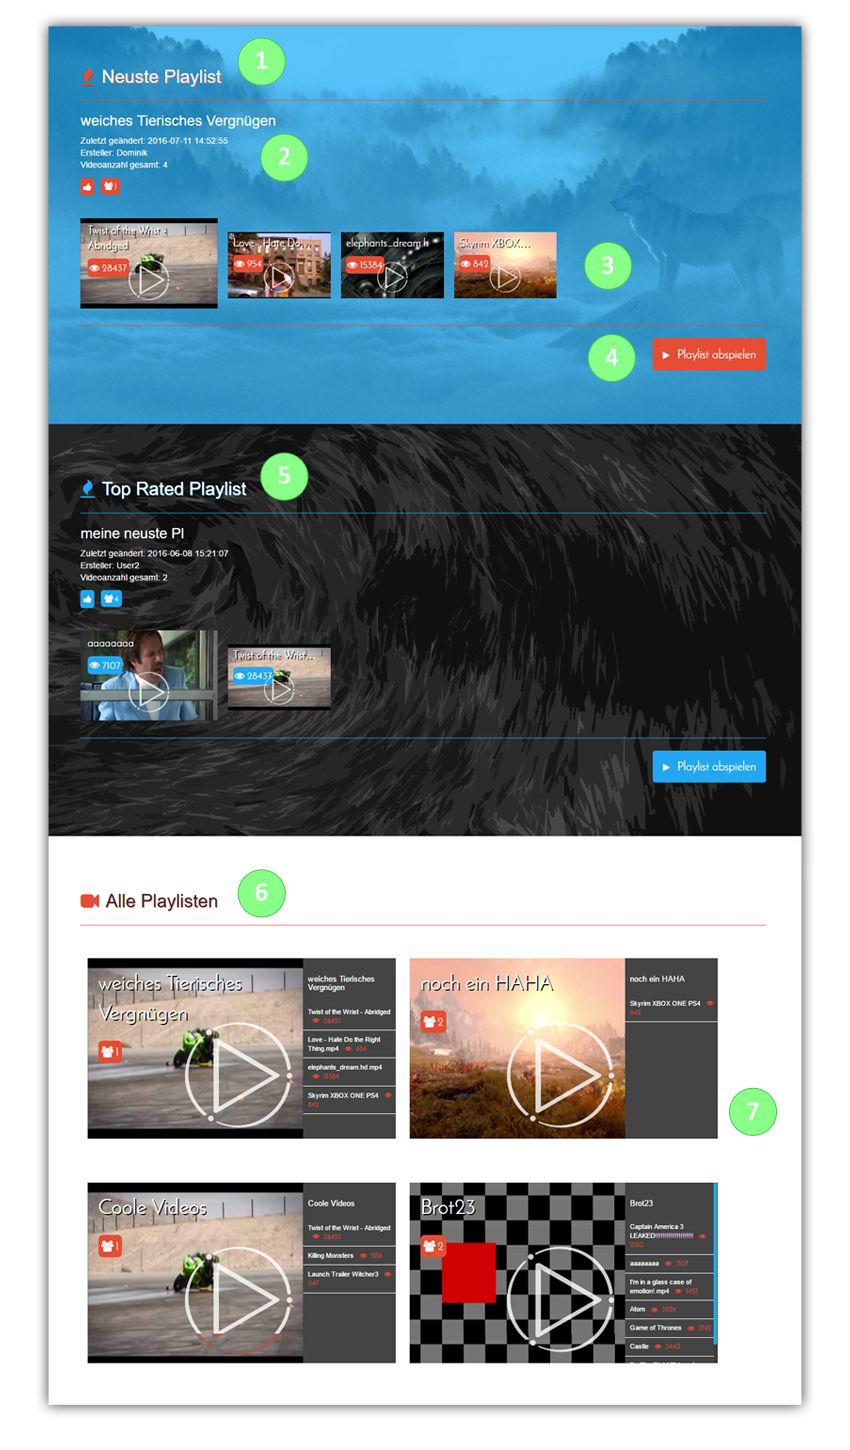
\includegraphics[width=0.95\textwidth]{./Includes/Bedienungsanleitung/playlist_nologin.png}
	\caption{Ansicht Playlists: ohne Login}
	\label{fig:playlist}

\end{figure}
\clearpage

{\bf Übersicht zu Abbildung 3.15}
\begin{enumerate}
	\item Neuste Playlist: Darstellung der zuletzt angelegten Playlist.
	\item Informationen zur Playlist: Name, Ersteller, Änderungsdatum, Videoanzahl, Abonnenten
	\item Auflistung der maximal ersten 5 Videos der Playlist. Über den Play-Button sind diese Videos einzeln abspielbar.
	\item Playlist abspielen: Link zur Playlist-Detailansicht der Playlist.
	\item Top Rated Playlist: Darstellung der Playlist mit dem höchsten Rating durch WolfGang-Nutzer. Der Aufbau dieser Ansicht verhält sich analog zu ''Neuste Playlist'', wie in den Punkten 2. - 4. beschrieben.
	\item Alle Playlisten: eine Übersicht zu den Playlisten ohne weitere Filter. Über den Play-Button oder den Link ''zur Playlist'' wird man auf die entsprechende Playlist-Detailseite weitergeführt. Die Videos einer Playlist werden rechts neben dem Vorschaubild (1. Video der Playlist) mit Scrollfunktion  gelistet.
\end{enumerate}


\begin{figure}[h!]
	\centering
	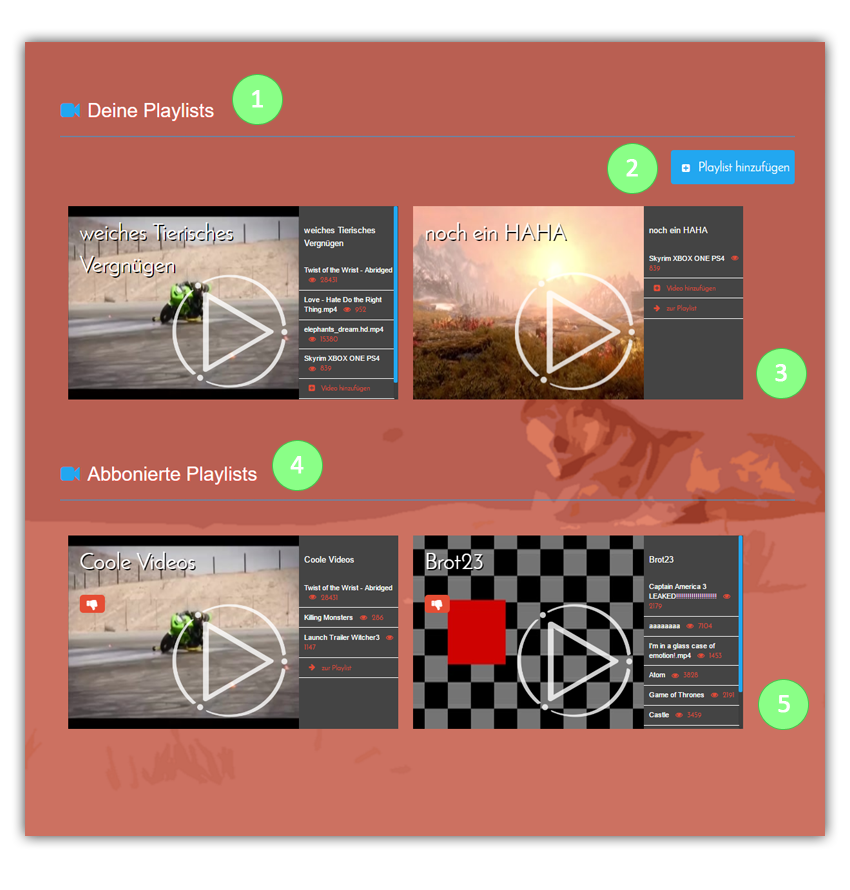
\includegraphics[width=1\textwidth]{./Includes/Bedienungsanleitung/playlist_login.png}
	\caption{Ansicht Playlists: nach Login}
	\label{fig:playlist-login}
\end{figure}

{\bf Übersicht zu Abbildung 3.16}
\begin{enumerate}
	\item Deine Playlists: Auflistung der vom angemeldeten Nutzer erstellten Playlisten.
	\item Playlist hinzufügen: öffnet ein Overlay zum Erstellen einer neuen Playlist.
	\item Playlist Ansicht: über den Play-Button oder den Link ''zur Playlist'' wird man auf die entsprechende Playlist-Detailseite weitergeführt. \\
	Die Videos der Playlist werden rechts neben dem Vorschaubild (1. Video der Playlist) mit Scrollfunktion gelistet. \\
	Über den Link ''Video hinzufügen'' können Videos per Suchfunktion hinzugefügt werden (siehe dazu: Videos zu Playlist hinzufügen).
	\item Abonnierte Playlists: Übersicht aller Playlisten, die vom angemeldeten Benutzer abonniert markiert wurden (per Like-Button).
	\item Playlist Ansicht: über den Play-Button oder den Link ''zur Playlist'' wird man auf die entsprechende Playlist-Detailseite weitergeführt. \\
	Die Videos der Playlist werden rechts neben dem Vorschaubild (1. Video der Playlist) mit Scrollfunktion gelistet. \\
	Mit dem ''Dislike''-Button kann das Abonnement für die Playliste beendet werden.
\end{enumerate}


\paragraph{Videos zu Playlist hinzufügen}
$\;$ \\ \\
Videos können zu einer Playlist auf zwei Wegen hinzugefügt werden. Entweder in der Video Detailansicht (siehe \hyperref[fig:video-detail]{''Video bearbeiten''}) oder unter Playlists, im Inhaltsbereich \hyperref[fig:playlist-login]{''deine Playlists''} mithilfe des Link ''Video hinzufügen''.

\begin{figure}[h!]
	\centering
	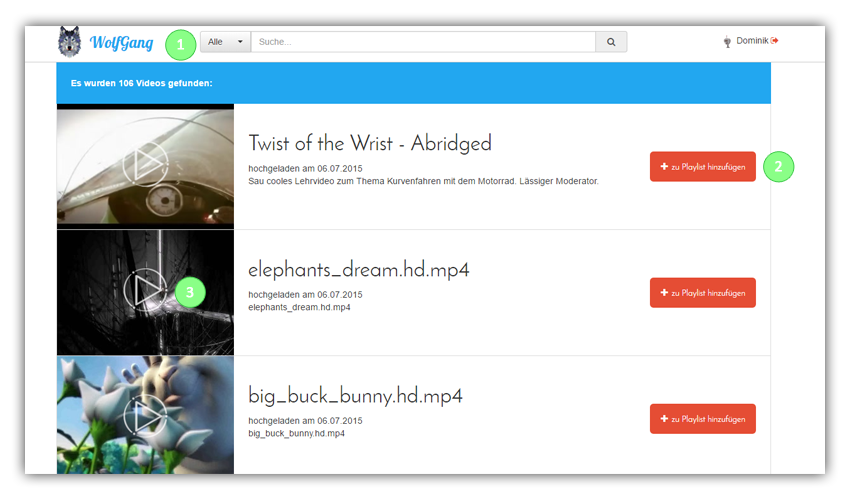
\includegraphics[width=1\textwidth]{./Includes/Bedienungsanleitung/playlist_addvideo.png}
	\caption{Ansicht Suchfunktion: Video zu Playlist hinzufügen}
	\label{fig:somthing}
\end{figure}

{\bf Übersicht zu Abbildung 3.17}
\begin{enumerate}
	\item Suchfunktion: um ein spezielles Video der gewählten Playlist hinzuzufügen kann es über die Suchfeld gesucht werden. Dabei muss bei der Auswahl entweder ''Alle'' oder ''Video'' hinterlegt sein (\it{diese Funktion ist aktuell leider fehlerhaft, da sie bis zum Abgabetermin nicht vollständig fertiggestellt werden konnte}).
	\item Button ''zu Playlist hinzufügen'': fügt das Video der gewählten Playlist hinzu. Man wird auf die Seite Playlists weitergeleitet.
	\item Video Wiedergabe
\end{enumerate}

\clearpage
\begin{figure}[h!]
	\centering
	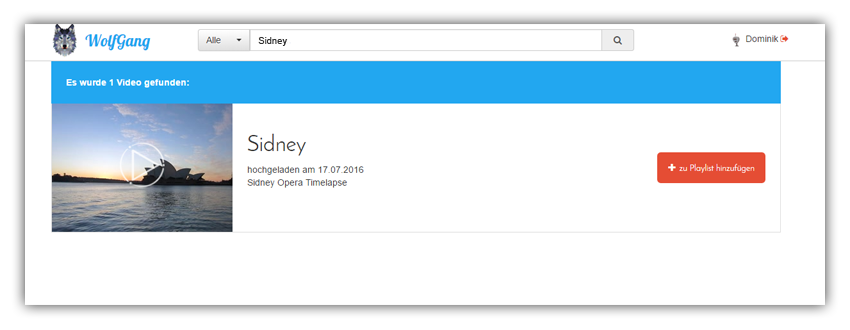
\includegraphics[width=1\textwidth]{./Includes/Bedienungsanleitung/playlist_addvideo2.png}
	\caption{Ansicht Suchfunktion: Video zu Playlist hinzufügen, nach Suche nach Video Sidney}
	\label{fig:somthing}
\end{figure}


\paragraph{Playlist Detailseite}
$\;$ \\ \\
Auf der Detailseite einer Playlist kann diese abgespielt und bearbeitet werden.

\clearpage
\begin{figure}[h!]
	\centering
	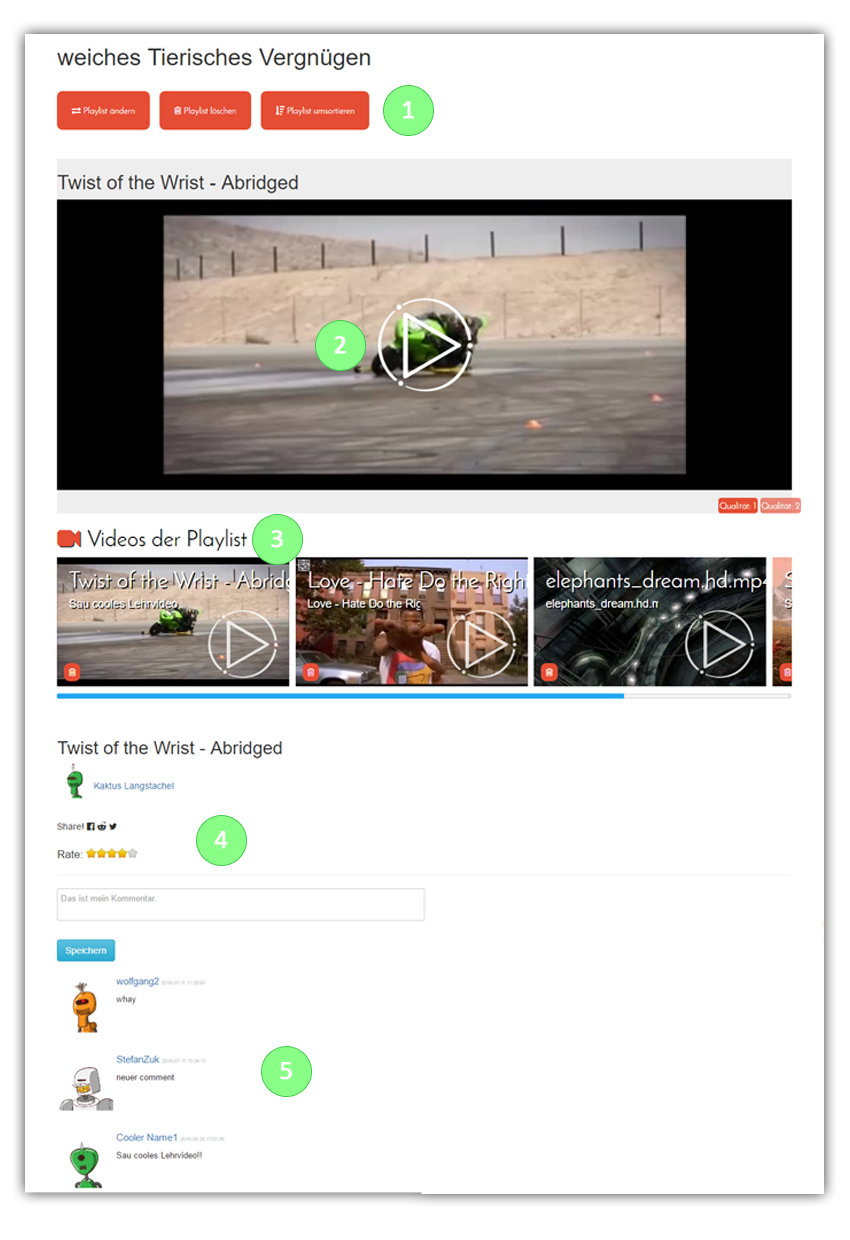
\includegraphics[width=1\textwidth]{./Includes/Bedienungsanleitung/playlistdetail.png}
	\caption{Ansicht Playlist Detailansicht}
	\label{fig:somthing}
\end{figure}

{\bf Übersicht zu Abbildung 3.19}
\begin{enumerate}
	\item Playlistname und Buttons zur Bearbeitung. Die Buttons können nur vom Ersteller Playlist oder einem User mit Adminrechten genutzt werden:
	\begin{enumerate}
		\item ''Playlist ändern'': Name der Playlist ändern
		\item ''Playlist löschen'': Playlist löschen
		\item ''Playlist umsortieren'': führt zur Ansicht zum Sortieren der Videos der Playlist
	\end{enumerate}
	\item Wiedergabe der Playlist
	\item Anzeige der Videos der Playlist, beim Abspielen eines Videos wird die Playlist an dieser Stelle weiter abgespielt.
	\item Informationen zum aktuellen Video: Videoname, Uploader-Name, Rating
	\item Kommentarfunktion und Darstellung der Kommentare des aktuellen Videos.
\end{enumerate}
\clearpage
\subsubsection{Admin Funktionen}
Admins haben Zugriff auch besondere Funktionen um die Verwaltung im Frontend zu ermöglichen.
\paragraph{Nutzerverwaltung}~\\
Der nur als Admin einsehbare Menüpunkt ''Usermanagement'' führt auf die entsprechende Unterseite.\\
Hier kann ein Admin die registrierten User mit seiner UserId, sein Namen, seiner Email Adresse und der Anzahl der Playlisten/Videos einsehen (2) und folgende Funktionen nutzen:
\begin{itemize}
\item[(1)] Nach Usern suchen, dadurch kommt man auf eine Einzelansicht (5). Durch ein Suchen nach \texttt{:all} kommt man zurück zu allen Benutzern.
\item[(3)] Alle User außer Admins löschen
\item[(4)] Die User Gruppe von allen Usern außer Admins löschen
\end{itemize}
\begin{figure}[h!t]
\centering
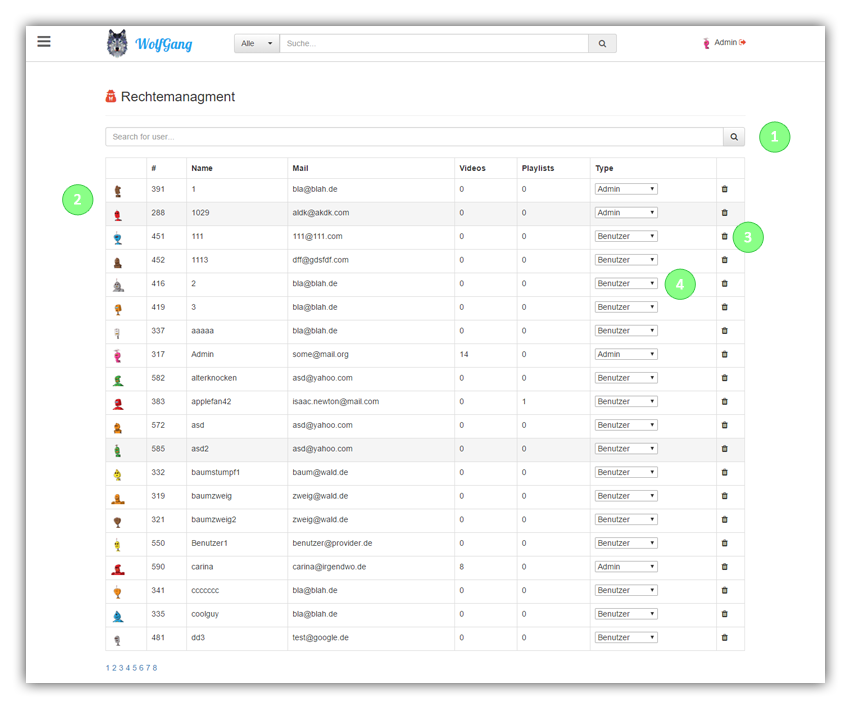
\includegraphics[width=\textwidth]{./Includes/Bedienungsanleitung/userma.png}
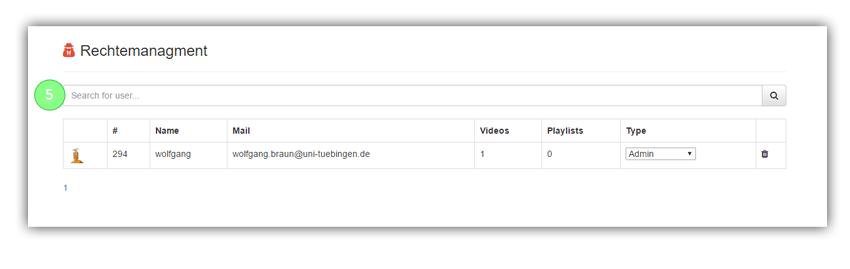
\includegraphics[width=\textwidth]{./Includes/Bedienungsanleitung/userma_search.png}
\end{figure}
\paragraph{Playlistverwaltung}~\\
Wenn ein Admin auf den Menüpunkt "Playlist" klickt, dann gelangt er statt zur normalen Useransicht, bei der Playlisten erstellt und angesehen werden können, zur Adminansicht, die zur Verwaltung der Playlisten verwendet wird (1). Neben einer Auflistung aller Playlisten werden folgende Funktionen zu Verfügung gestellt:
\begin{itemize}
\item[(2)] Der Name der Playlist geändert werden. Vergisst der Admin danach den Edit Knopf(3) zu drücken warnt ihn eine rote Umrandung vor
nicht gespeicherten Änderungen (4)
\item Jede Playlist kann gelöscht werden, egal wer sie erstellt hat (3)
\end{itemize}
\begin{figure}[h!t]
\centering
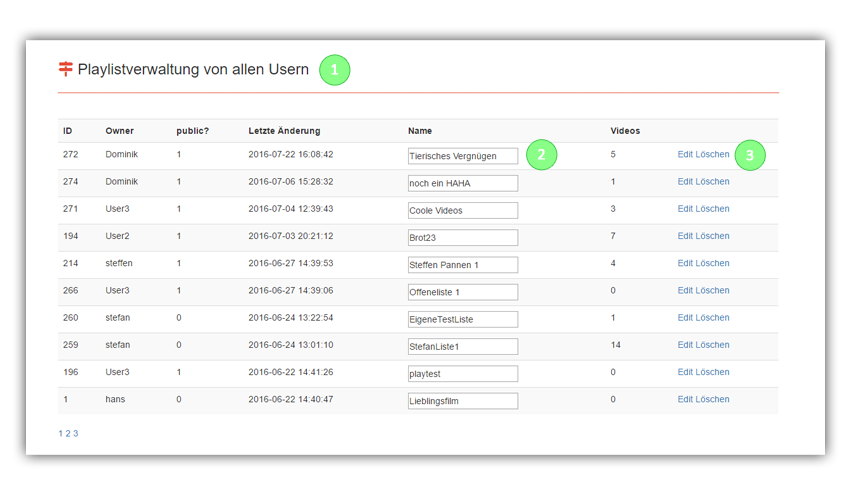
\includegraphics[width=\textwidth]{./Includes/Bedienungsanleitung/playlist_admin.png}
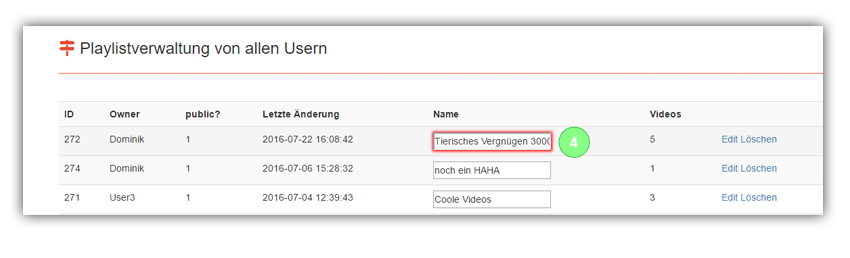
\includegraphics[width=\textwidth]{./Includes/Bedienungsanleitung/playlist_admin_edited.png}
\end{figure}
\paragraph{Kategorienverwaltung}~\\
Wenn ein Admin auf den Menüpunkt ''Kategorien'' klickt, erhält er ein leicht anderes Layout (1) als Nutzer der anderen Gruppen.\\
Hier wird die UserIds des Erstellers, der Name der Kategorie und die Anzahl der Videos angezeigt.\\
Außerdem kann ein Admin Kategorien umbenennen, löschen (3) und erstellen (2).
\begin{figure}[h!t]
\centering
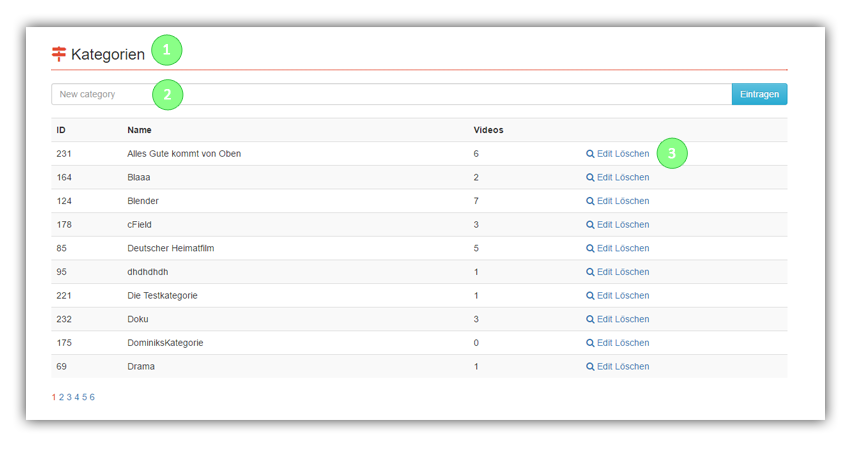
\includegraphics[width=\textwidth]{./Includes/Bedienungsanleitung/kategorien.png}
\end{figure}


\section{Probleme und Lösungen}
\label{probleme}
Grundsätzlich werden alle (Fehler-) Meldungen über eine Notify-Box rechts unten unmittelbar nach dem Ereignis eingeblendet um so über Erfolg oder Misserfolg der Aktion zu informieren.




\begin{enumerate}
\item \textit{Buttons funktionieren nicht(Drop-Down-Menü erscheint nicht)} : \\
Überprüfen sie, ob Javascript aktiviert ist.
\item \textit{Videos können nicht abgespielt werden}: \\
Überprüfen sie ob sie die aktuellen Treiber zur Wiedergabe eines .mp4 Videos über den HTMl5 Player installiert haben. \\
\item \textit{Elemente werden nicht dargestellt(Seite ist fast leer)} : \\
Vermutlich ist der Backendserver, der die meisten Daten liefert, gerade nicht erreichbar. Diesen Fehler können sie selbst nicht beheben, versuchen sie es später nochmal. \\
\item \textit{Ich kann ein Video/eine Playlist/eine Kategorie nicht finden:} \\
Die Suche erkennt leider keine ähnlichen Begriffe(oder ähnliche Schreibweisen): \\
Wollen sie eine Kategorie "Fisch" aufrufen, suchen aber nach "Fische", so werden sie die Kategorie nicht finden. Versuchen sie in diesem Fall die Suche mit einem Teilbegriff (und wählen das richtige Ziel über die Suchvorschläge aus). Finden sie trotzdem kein Ergebnis, so gibt es kein Ziel, wo den Suchbegriff als Teil ihres Namens besitzt. \\
\item \textit{Registrierung geht nicht} : \\
1. Bekommen sie die Fehlermeldung "Passwörter stimmen nicht überein", so geben sie ihr Passwort und die Bestätigung erneut ein (achten sie auf Groß/Kleinschreibung). \\
2. Bekommen sie eine Fehlermeldung über die Notify-Box, so ist entweder die angegebene E-Mail Adresse ungültig oder ihr Username wird bereits verwendet (genaue Informationen stehen in der Benachrichtigung). In diesem Fall müssen sie sich einen anderen Usernamen /eine gültige E-Mail Adresse eingeben. \\
\item \textit{Ich kann meinen Kommentar nicht bearbeiten}: \\
Eine Bearbeitung des Kommentars ist derzeit leider nicht möglich. Sie können allerdings ihren alten Kommentar löschen und einen neuen schreiben.  \\
\item \textit{Ich sehe die in der Anleitung beschriebenen Knöpfe nicht} : \\
Sind die Knöpfe nicht sichtbar, so haben sie nicht die benötigten Rechte, um die Aktionen, die mit den Knöpfen assoziiert sind, auszuführen. Schauen sie sich dafür  die \hyperref[Rechte]{Rechtetabelle} an. \\
\item \textit{Video Upload funktioniert nicht}: \\
Bekommen sie keine Fehlermeldung und das Video wird trotzdem nicht hochgeladen, so ist vermutlich die Größe des Videos größer als die vom Server erlaubte maximale Größe. Komprimieren sie ihr Video oder versuchen sie es mit einem kleineren Video. \\
\end{enumerate}

\section{Besonderheiten von WolfGang}

\subsection{Die Idee WolfGang}
Um dem Projekt einen Namen und ein Thema für das Design der Website zu geben, war beim Projektstart wichtig, eine passende Idee zu finden. Dabei stand die Namensfindung im Mittelpunkt. \\
Der Name ''WolfGang'' entstand mit der Anlehnung an den Trend, Software nach einem deutschen Namen zu benennen, wie z.B. beim Messenger ''Franz''. Als Name wurde der, des Projekt Betreuers Wolfgang Braun gewählt - auch da sich damit ein Themenfeld für Design und Konzeption anboten. Das Thema ''Wolf'' ist das Design-Thema und grafisch überall auf der Website zu finden, wobei ''Gang'' für einen Rundgang durch die Videos der Plattform stehen soll. \\

\begin{figure}[h!]
	\centering
	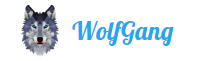
\includegraphics[width=0.33\textwidth]{./Includes/Bedienungsanleitung/logo.png}
	\caption{Logo WolfGang}
	\label{fig:somthing}
\end{figure}

\subsection{Navigation und Overlay Techniken}
Durch die Overlay Technik konnten viele Funktionen der Website grafisch sinnvoll und einfach eingebunden werden, ohne dass der Übersicht für den Nutzer der Website gestört wird. Beispiele hierfür sind die Hauptnavigation, sowie Buttons für Video- und Playlist-Verwaltung.

\begin{figure}[h!]
	\centering
	\begin{minipage}{0.49\textwidth}
		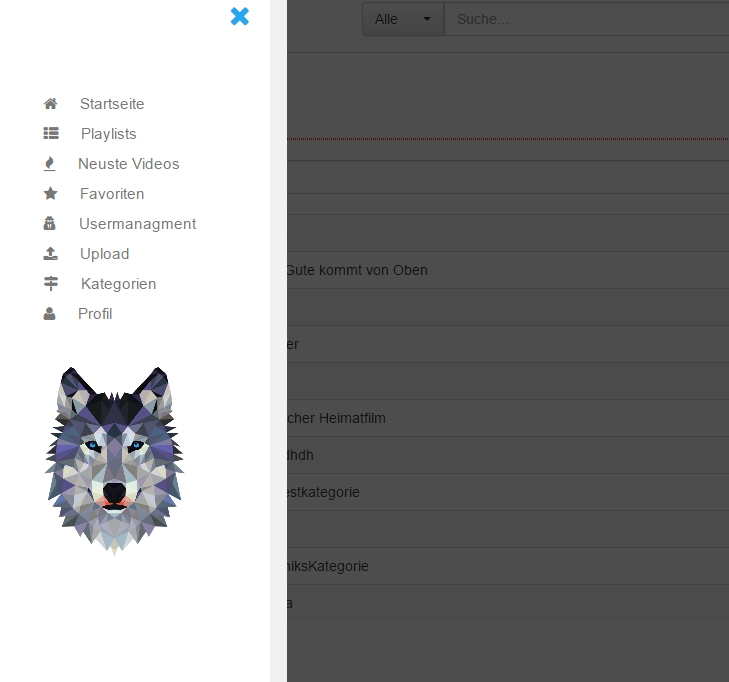
\includegraphics[width=0.95\textwidth]{./Includes/Bedienungsanleitung/specials_navi_overlay.png} 
	\end{minipage}%
	\begin{minipage}{0.49\textwidth}
		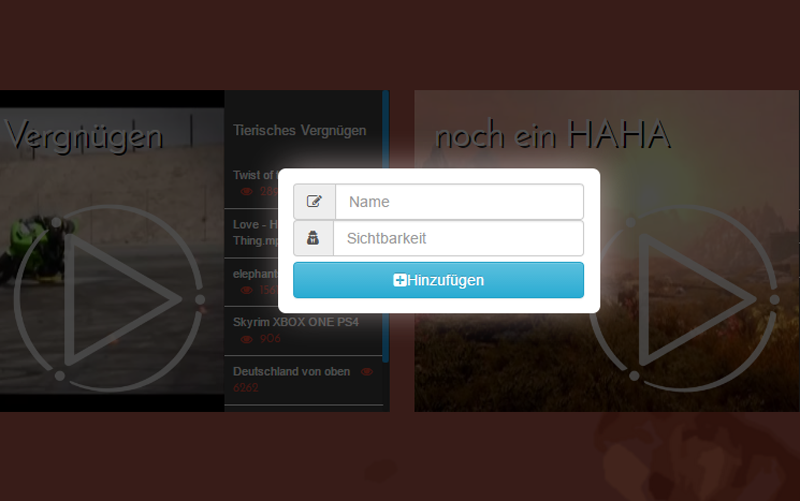
\includegraphics[width=0.95\textwidth]{./Includes/Bedienungsanleitung/specials_overlay.png}
	\end{minipage}
	\caption{Overlay Ansicht Hauptnavigation / Button-Funktion}
	\label{fig:somthing}
\end{figure}


\subsection{Wolf-Design}
Angelehnt an den Projektnamen ist der Wolf, als Logo und Symbol für das Projekt an zahlreichen stellen der Website zu finden und kennzeichnet das Design der Website. Genutzt wurden dafür ausschließlich freie Grafiken (Bilder, Gifs, Vektorgrafiken), die ggf. noch nachträglich abgewandelt, bearbeitet und für die Seite aufbereitet wurden. Beispiele finden sich dafür unter anderem im Logo, der Navigation, in den Hintergrundgrafiken des Content-Bereichs und der 404-Seite. 

\begin{figure}[h!]
	\centering
	
\includegraphics[width=0.33\textwidth]{./Includes/Bedienungsanleitung/wolf_v2.png}
	\caption{Logo Image}
	\label{fig:somthing}
\end{figure}

\begin{figure}[h!]
	\centering
	\begin{minipage}{0.33\textwidth}
		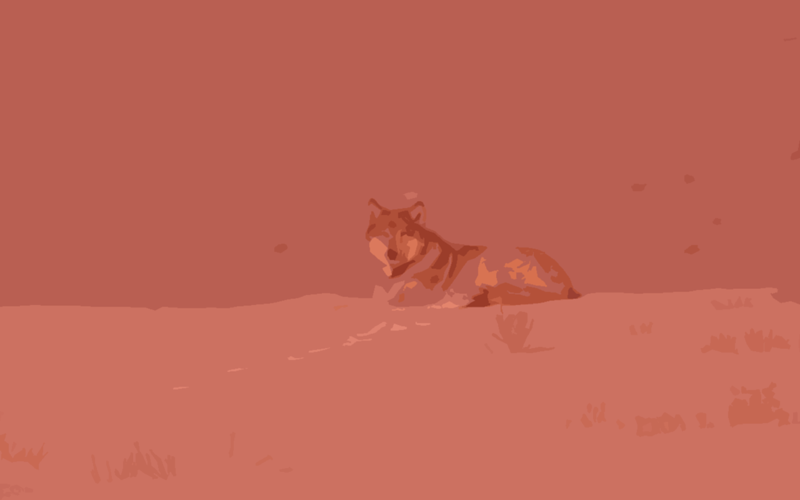
\includegraphics[width=0.95\textwidth]{./Includes/Bedienungsanleitung/wolf_red.png} 
	\end{minipage}%
	\begin{minipage}{0.33\textwidth}
		
\includegraphics[width=0.95\textwidth]{./Includes/Bedienungsanleitung/wolf_blue.png}
	\end{minipage}%
	\begin{minipage}{0.33\textwidth}
		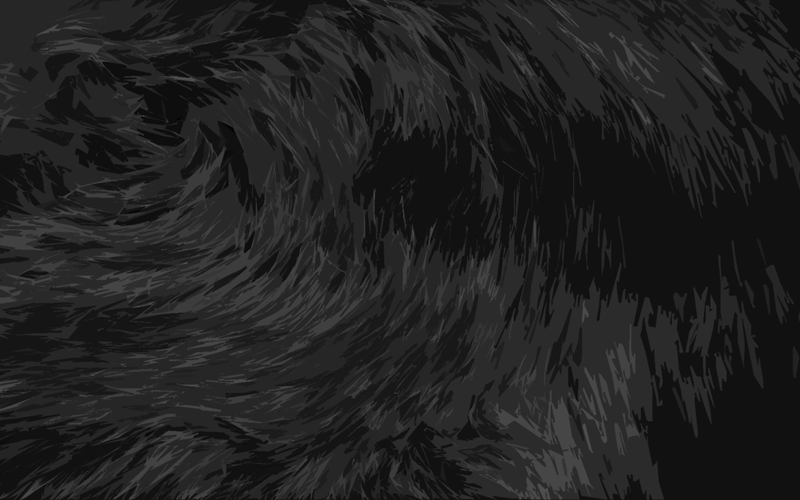
\includegraphics[width=0.95\textwidth]{./Includes/Bedienungsanleitung/wolf_black.png}
	\end{minipage}
	\caption{Hintergründe (rot, blau, schwarz)}
	\label{fig:somthing}
\end{figure}


\subsection{Tag Cloud Kategorien}
Eine Begriffs-Wolke mit zufälligen Kategorien-Namen. Kategorien mit vielen Videos werden groß dargestellt, Kategorien mit wenigen Videos kleiner.

\begin{figure}[h!]
	\centering
	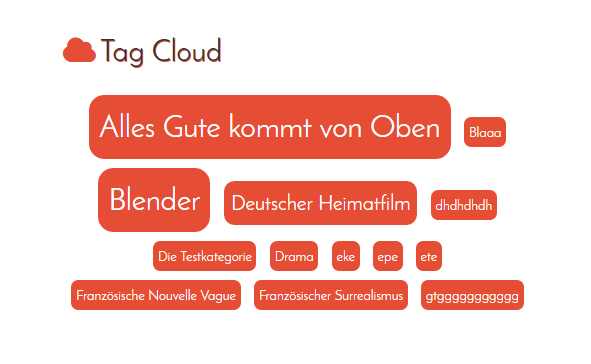
\includegraphics[width=1\textwidth]{./Includes/Bedienungsanleitung/catcloud.png}
	\caption{Category Cloud}
	\label{fig:somthing}
\end{figure}

\subsection{RoboHash: automatische Benutzerbilder}
Da das Backend keine Avatar Funktionen anbietet, wurde RoboHash.org für die Generation zufälliger Benutzerbilder für jeden User verwendet.

\begin{figure}[h!]
	\centering
	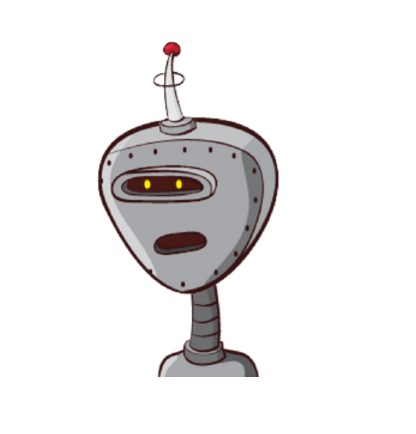
\includegraphics[width=0.33\textwidth]{./Includes/Bedienungsanleitung/robot.png}
	\caption{RoboHash Profilbild}
	\label{fig:somthing}
\end{figure}

\subsection{Typeahead Suchfunktion}
Durch ein Bootstrap Addon ist die Suche mit dem ''Typeahead'' Feature ausgestattet. Beim tippen wird direkt die Suche im Hintergrund ausgeführt.

\begin{figure}[h!]
	\centering
	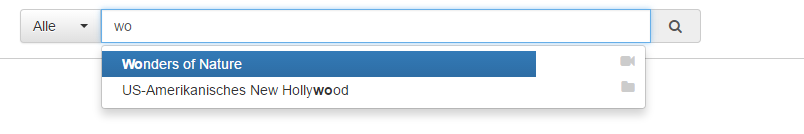
\includegraphics[width=1\textwidth]{./Includes/Bedienungsanleitung/autocomplete.png}
	\caption{Autocomplete Beispiel der Suchfunktion}
	\label{fig:somthing}
\end{figure}



\end{document}